\section{Project Planning and Timeline}

The overall project will span a total of two academic semesters of the senior year (a total of approximately 8 months) and will comprise a set of goals for each semester. The project will be managed using an agile methodology, where by the end of the project, two deliverables will be obtained: MVP1 and MVP2. This section will break down the project planning and timeline for each MVP, as well as expected deliverables for each phase.

\subsection{Channels}

Throughout the project, two essential tools will be used to facilitate communication and task delegation within the project. The first tool is Discord, a multi-functional communication tool that is practical for meetings, scheduling events, and so on. Discord will be used as the primary communication tool for the members in the project, as well as for some advisors. The second tool is Jira, an agile project management tool that facilitates task delegation and software project management. Jira will be used to track the tasks of each member in the project, as well as to track software features and bugs within the project in the form of tickets for ease of audit. Additionally, it will also comprise the customer journey of each feature of the robot in the form of “user stories.”

\subsection{MVP 1 - Proof of Concept \& Customer-Centric Specifications}

MVP 1 will span the entirety of academic semester 1 (from September until December) and will focus on delivering a proof of concept of the project, as well as feature specifications that focus on the customers’ needs. MVP 1 will comprise three sprints, each lasting for around a month.

The project starts at MVP 1 Sprint 0, which focuses on preliminary research and feature definition. This sprint will span the entirety of September, and comprises the project proposal, in-depth customer journey, and technology specifications (such as specifically which AI models to be used). MVP 1 Sprint 0 will have two deliverables: the written project proposal and first progress report.

In the next phase, MVP 1 Sprint 1, which lasts from October to early November, we will focus on preliminary software development aimed towards providing a proof of concept for the emotion detection algorithm. For each AI model that will be used, we will allocate time for data collection, training, and iterative quality checks using real data. In general, emotion detection will comprise detection of facial expressions, Speech Emotion Recognition (SER), and Gesture Recognition technologies, utilizing computer vision and feature extraction technologies. In addition, there are plans to integrate context understanding into the robot using NLP technologies, but we will not include it in the scope. Additionally, the UX design will also be drafted, consisting of a complete customer journey for each feature, as well as a basic outer shell for the robot that fits the design specifications. Sprint 1 will have three deliverables: second progress report, third progress report, and completed prototypes for emotion detection.

In the last phase, MVP 1 Sprint 2, which lasts from November to early December, we will focus on acquiring the first batch of hardware components for the project and testing the emotion detection models on our selected microcontroller. The microcontroller must have enough compute power to perform inferences in real time. Additionally, Sprint 2 will involve market validation, which comprises testing on the customer segment to obtain feedback for improvement in the following semester. By the end of MVP 1, we expect a prototype that integrates software and hardware components on a feasible level.

\begin{figure}[ht]
    \centering
    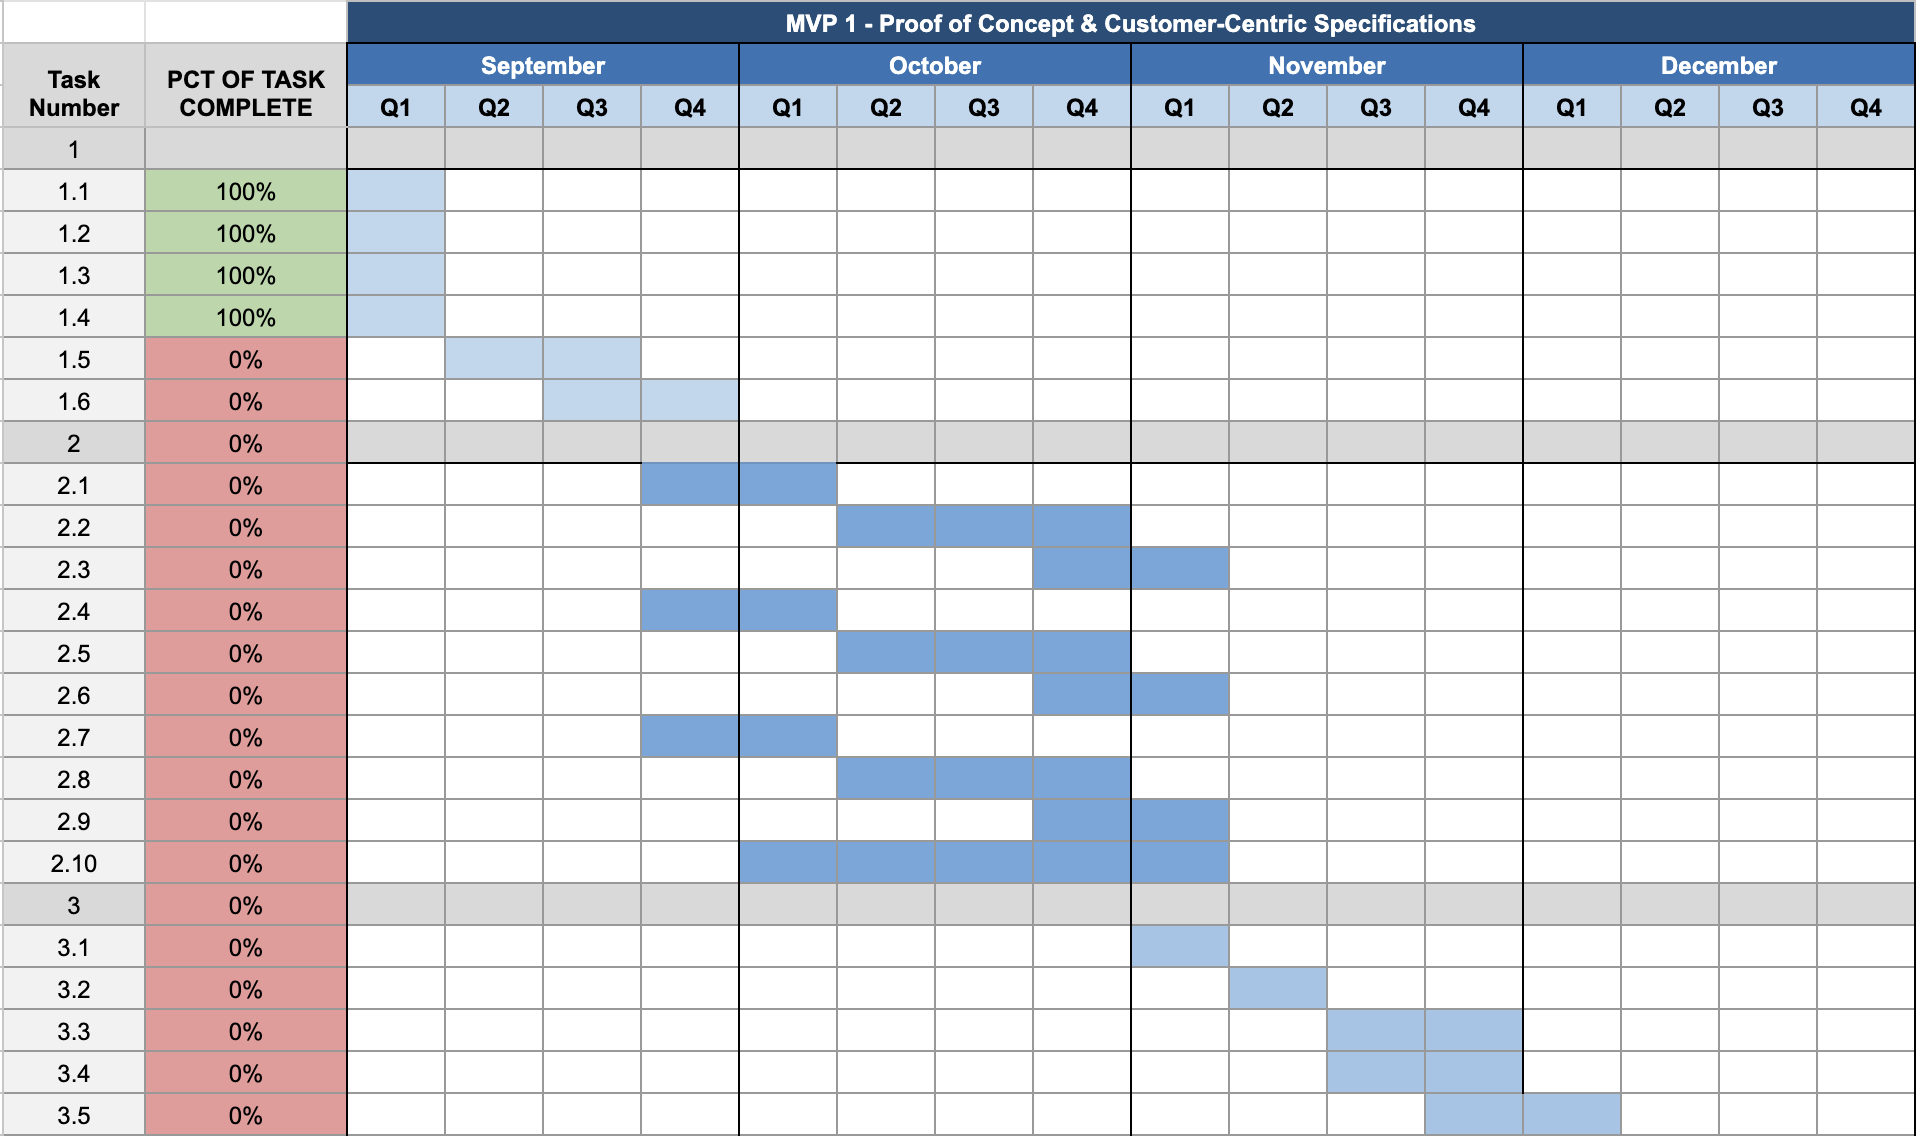
\includegraphics[width=\textwidth]{gantt-table.png}
    \caption{Gantt Chart for MVP 1 Timeline}
    \label{fig:gantt}
\end{figure}
\newpage
\subsection*{Task Number:}
\begin{enumerate}
\item\textbf{MVP 1 - Sprint 0}\\
1.1	Advisor Onboarding\\
1.2	Project Scoping\\
1.3	Project Scoping - Expert Interviews\\
1.4	Project Proposal\\
1.5	In-Depth Technology Specifications\\
1.6	E2E Customer Journey\\
\item\textbf{MVP 1 - Sprint 1}\\
2.1	Facial Expression Model - Data Collection\\
2.2	Facial Expression Model - Training/Testing\\
2.3	Facial Expression Model - Quality Testing\\
2.4	SER Model - Data Collection\\
2.5	SER Model - Training/Testing\\
2.6	SER Model - Quality Testing\\
2.7	Gesture Model - Data Collection\\
2.8	Gesture Model - Training/Testing\\
2.9	Gesture Model - Quality Testing\\
2.10 UX Design (Fusion360)\\
\item\textbf{MVP 1 - Sprint 2}\\
3.1	Parts Procurement\\
3.2	Jetson Orin/Nano Test\\
3.3	MVP 1 Integration \\
3.4	Market Validation\\
3.5	Final Presentation Preparations\\
\end{enumerate}

\newpage
\subsection{MVP 2 - Non-Commercial Prototype}

In this project proposal, the specific details of MVP 2 will not be disclosed. However, in general, MVP 2 will comprise three sprints, similar to MVP 1, but will focus on integration of the emotion detection algorithm with hardware components to create an output. MVP 2 will last the entirety of academic semester 2, and is expected to deliver a fully functional prototype, but will not be implemented to the extent of commercialization. Additionally, MVP 2 will focus on user testing, involving measurable metrics mentioned in the objectives section. The prototype will not encompass full consideration of security, safety, and real usage, but will focus on fulfilling the customer demands of appearance, interactivity, and empathy.

\subsection{Resource Allocation}

The project team comprises three senior engineering students. The roles for the project will be designated as follows: project manager, project engineer for product development, and project engineer for software development. The project manager is responsible for overseeing the entire project, delegating tasks, managing the timeline, and creating engagements with advisors from ISE and Chula Student Wellness. They are expected to streamline work processes for the project engineers and professionally check deliverables before submission. The project engineers are separated into two categories: product development and software development. The product development engineer will be responsible for UX design through CAD software, gathering hardware components, and managing the budget for doing so. The software development engineer will be responsible for overseeing all software initiatives, as well as managing DevOps practices within the project.

\subsection{Budget Allocation}

While the exact hardware components for the robot cannot be deduced yet, the table below will illustrate an approximate allocation of the budget provided for the project. Note that the budget specified is the maximum that was allocated for expenditure. The budget for each component may vary, but should never exceed the maximum allocated budget.

\begin{table}[ht]
\centering
\begin{tabular}{|l|l|}
\hline
\textbf{Component} & \textbf{Maximum Allocated Budget (THB)} \\ \hline
Microcontroller & 30,000 \\ \hline
Camera & 5,000 \\ \hline
Microphone & 5,000 \\ \hline
Electronics & 15,000 \\ \hline
Chassis and Framework & 5,000 \\ \hline
Decorative Components & 5,000 \\ \hline
LED Display & 5,000 \\ \hline
Miscellaneous & 5,000 \\ \hline
\textbf{Maximum Expenditure} & \textbf{75,000} \\ \hline
\end{tabular}
\caption{Approximate Budget Allocation for Hardware Components}
\end{table}
